\documentclass[a4paper,12pt,oneside]{report}
\usepackage[english]{babel}      % česky psaná práce
\usepackage[T1]{fontenc}
%\usepackage[cp1250]{inputenc}  % vstupní znaková sada: Windows 1250
\usepackage[utf8x]{inputenc}  % vstupní znaková sada: ISO Latin 2

\usepackage{amsmath} % balíček pro pokročilou matem. sazbu
\usepackage{amssymb}
\usepackage{epsfig} % balíčky pro vkládání grafických souborů typu EPS
\usepackage{listings}
\usepackage{xcolor}
\usepackage{url}
\usepackage{colortbl}
\usepackage{caption}
\usepackage{pdfpages}
\usepackage{hyperref}

\DeclareMathOperator*{\argmin}{\arg\!\min}
\DeclareMathOperator*{\argmax}{\arg\!\max}
\DeclareCaptionFont{white}{ \color{white} }
\DeclareCaptionFormat{listing}{
  \colorbox[cmyk]{0.43, 0.35, 0.35,0.01 }{
    \parbox{142mm}{\hspace{15pt}#1#2#3}
  }
}

\captionsetup[lstlisting]{format=listing, labelfont=white, textfont=white, singlelinecheck=false, margin=0pt, font={bf,footnotesize} }
\lstset{frame=single, texcl=true, breaklines=true, morecomment=[l]{//}, backgroundcolor=\color{red!10!green!10!blue!5!}}
\renewcommand{\lstlistingname}{Ukázka kódu}
%\usepackage{graphicx} % balíček pro vložení grafických souborů typu JPG -- přeložte pomocí PDFtex!

%\usepackage{fancybox} % umožňuje pokročilé rámečkování :-)
%\usepackage{index} % nutno použít v~případě tvorby rejstříku balíčkem makeindex

%\newindex{default}{idx}{ind}{Rejstřík} % zavádí rejstřík v~případě použití balíku index


%\oddsidemargin=10mm   % levý okraj větší (kvůli vazbě)
%\evensidemargin=0mm
\topmargin=-15mm      % horní okraj trochu menší
%\textwidth=150mm      % šířka textu na stránce
\textheight=240mm     % "výška" textu na stránce


\pagenumbering{arabic} % číslování stránek arabskými číslicemi
\pagestyle{plain}      % stránky číslované dole uprostřed

\parindent=0pt % odsazení 1. řádku odstavce
\parskip=7pt   % mezera mezi odstavci
\frenchspacing % aktivuje použití některých českých typografických pravidel

% definice makra pro české uvozovky:
\def\bq{\mbox{\kern.1ex\protect\raisebox{-1.3ex}[0pt][0pt]{''}\kern-.1ex}}
\def\eq{\mbox{\kern-.1ex``\kern.1ex}}
\def\ifundefined#1{\expandafter\ifx\csname#1\endcsname\relax }%
\ifundefined{uv}%
        \gdef\uv#1{\bq #1\eq}
\fi
% konec .... použití makra pro psaní český uvozovek: \uv{text uvnitř uvozovek}


%%%%%%%%%%%%%%%%%%%%%% zde jsou zavedeny některé "konstanty" - můžete, resp. musíte je ZMĚNIT %%%%%%%%%%%%%%%%%%%%%%
\newcommand{\cvut}{Czech Technical University in~Prague}
\newcommand{\fjfi}{Faculty of Nuclear Sciences and Physical Engineering}
\newcommand{\kse}{}
\newcommand{\obor}{}
\newcommand{\zamereni}{}

\newcommand{\nazevcz}{Počítačové adaptivní testování}        % zde VYPLŇTE český název práce (přesně podle zadání!)
\newcommand{\nazeven}{Probabilistic Models for Computerized Adaptive Testing}     % zde VYPLŇTE anglický název práce (přesně podle zadání!)
\newcommand{\autor}{Ing. Martin Plajner}           % zde VYPLŇTE své jméno a příjmení
\newcommand{\rok}{2016}                % zde VYPLŇTE rok odevzdání, např. 2006
\newcommand{\vedouci}{Ing. Jiří Vomlel, Ph.D.}         % zde VYPLŇTE jméno a příjmení vedoucího práce, včetně titulů
                                                               % např. Doc. Ing. Ivo Malý, Ph.D.
\newcommand{\pracovisteVed}{\kse, \fjfi, \cvut} % zde VYPLŇTE pracoviště vedoucího práce, je-li jiné než KSE FJFI ČVUT

\newcommand{\konzultant}{---} % POKUD MÁTE určeného konzultanta, NAPIŠTE jeho jméno a příjmení
\newcommand{\pracovisteKonz}{} % POKUD MÁTE konzultanta, NAPIŠTE jeho pracoviště


\newcommand{\klicova}{počítačové, adaptivní, testování, bayesovské sítě}   % zde NAPIŠTE česky max. 5 klíčových slov
\newcommand{\keyword}{computerized, adaptive, testing, Bayesian networks}       % zde NAPIŠTE anglicky max. 5 klíčových slov (přeložte z~češtiny)
\newcommand{\abstrCZ}{} % zde NAPIŠTE abstrakt v~češtině
\newcommand{\abstrEN}{Abstract}                  % zde NAPIŠTE abstrakt v~angličtině



\begin{document}


\thispagestyle{empty}

\begin{center}
    {\Large \bf \cvut\\[2mm] \fjfi }
    \vspace{10mm}

    \begin{tabular}{c}
    {\bf \kse}\\
    \end{tabular}

   % logo CVUT -- pokud jej nechcete použít, zakomentujte následující řádek a odkomentujte řádek pod ním:
      \vspace{10mm}
    \centering{
\includegraphics[height=25mm]{cvutlogobw.png}}
    \vspace{10mm}
   %\vspace{50mm}

   {\Huge \bf \nazeven}

   
   {\Large Study for dissertation thesis}
  {\center \textbf{Abstract:} } \\
	\abstrEN  \\
  {\em Key words:} 
	{\keyword}
   \vfill
   {\large
    \begin{tabular}{rl}
    Author: & \autor\\
    Supervisor: & \vedouci\\
    Year: & \rok
    \end{tabular}
   }
\end{center}

\newpage  
\tableofcontents 

\newpage % SEM NESAHEJTE!

\chapter*{Introduction} \addcontentsline{toc}{chapter}{Introduction} 
\chapter*{Introduction} \addcontentsline{toc}{chapter}{Introduction} 
Educational testing is an important part of our lives in the modern society. Every person participates in a large number of tests which are used to assess his/her level of knowledge, quality, or skill in a certain domain. There are many different possibilities how to design a test for a specific purpose. The theory of test creation, administration, validation, etc. (in general called psychometrics) is extensive (for example,~\cite{1964psychometrics, Lord, Rasch1981, Mislevy1994}, and many others). The process of the creation of a good test is long, contains many steps, and can be performed in many different ways. In the classical approach we first identify the target ability (the ability we want to measure). Afterwards, there are repeated cycles of adding new questions, testing the test on a small set of examinees (to see if the questions are measuring the right ability in a correct way), and removing unsuitable questions. In the end we end up with one satisfactory version of the test. This test is fixed in its questions (i.e. every student taking the test will have the same questions). This approach does not take into account the individuality of each examinee. It is clear that for a skilled examinee the test will necessarily contain a lot of questions which are too easy and vice versa. The time which is being spent by solving these questions could be used to better differentiate his/her skill. This can be achieved by asking questions with an appropriate difficulty.
 
There are banks of questions which are suitable to measure the ability of a student (sometimes they are quite limited – for example if we measure a physical ability there might be a limited number of possible questions – and sometimes they are unlimited – in mathematics we can create as many different problems to solve as we want to). Questions for a test are selected from this bank. If we use one set of questions for every test there will be a lot of possibly good questions which are never asked (those which remained in the question bank unselected). The same set of questions for every test also, in some cases, encourages cheating (which of course can usually be solved by other methods, but it requires additional steps). Some tests do not follow the outline explained in the paragraph above and tries to utilize the whole bank of questions. One way of doing that is for example used in the Czech driving license test~\cite{Dopravy2006}. It is a computer test where 25 questions are randomly selected from approximately a thousand of possible questions. This approach negates the possibility of learning all the questions by heart as well as cheating by looking into your neighbor’s sheet. A test in a similar manner is done by a Faculty of Medicine of the Charles University~\cite{UK} as an entrance exam test. Questions for the entrance exam are selected from a set (book) of possible questions for each test (i.e., question bank). Several versions of a test are prepared for every entrance exam session. Both of these selection processes (driver’s license and entrance exam) remove some complications mentioned above but produce new problems. In the driver’s license test, where the question selection is done automatically by the system, it is hard to ensure the overall difficulty of each test will be approximately the same. Cases where a lot of easy questions or on the contrary a lot of difficult questions is selected might occur. In the approach of medical faculty this unfair combination can be avoided by a careful test composition. The test composition is done by hand by specialists but these specialists sometimes have shifted notion of the difficulty of individual questions (some things they may think of as very easy are actually hard for young students). There is also definitely a lot of effort and time involved in the preparation of every entrance exam round.

Computerized Adaptive Testing (CAT) offers a way to overcome some of the limitations given by the classical testing approach. The examinee is answering questions presented to him/her by a computer system. This system is centered on a student model. There are many ways to construct a student model. One way is a model composition by experts. Another is to construct the model from a data set of many previously tested examinees. These examinees have to be tested without the adaptive approach to obtain a basis for the model creation. Afterwards, the model can be further updated and extended with new cases even while being in use. During the course of testing the student model is updated to reflect abilities of the tested student and as a part of that process an estimation of student’s level of knowledge is updated as well. This provides us an actual estimation of student’s abilities in every phase of testing. At the same time the model is used to select a next question. The next selected question is the most appropriate one. An appropriate question suits certain criteria, usually providing the best information about the student at the current stage of testing. Questions are selected from a bank of questions. This bank can be similar to an question bank for the classical test. Adaptive testing is performed until a criterion is reached. There is a variety of possible criteria; usually we want to stop the test when the confidence of the estimation of student’s skill is above a certain significant value. Other practical limitations might affect this criterion such as the total time of a test or the number of asked questions. The adaptive testing concept brings many advantages but also some disadvantages over the classical testing approach. These aspects are detailed in the following chapters. Further we present different model types and perform experiments with our empiric data.
 

\chapter{Computerized Adaptive Testing}
This chapter introduces the concept of Computerized Adaptive Testing (CAT) and summarizes its advantages and disadvantages.
 
CAT is a concept of testing which is getting large scientific attention for about two decades~\cite{Linden2000, Wainer1990, VanderLinden2010}. With CAT we build computer administered and computer controlled tests. The computer system is selecting questions for a student taking the test and evaluating his/her performance. 


The process can be divided into two phases: model creation and testing. In the first one the model of the student is created while in the second one the model is used to actually test examinees. There are many different model types which can be used for adaptive testing. In this work we are going to cover Item Response Theory (IRT), which is a model regularly used for CAT, Bayesian networks, and Neural Networks, which are both models commonly used in many areas of artificial intelligence for a large variety of tasks. We will pay closer attention to these models later on but regardless of the model we choose the testing part follows always the same scheme. With the prepared and calibrated model, CAT testing repeats following steps.

\label{sec:CATprocess}
\begin{itemize}
	\item The next question to be asked is selected.
	\item This question is asked and an answer is obtained.
	\item This answer is inserted into the model.
	\item The model (i.e., our estimation about the student's skill) is updated.
	\item (optional) Answers to remaining question are estimated
\end{itemize}

This procedure is repeated until we reach a termination criterion. There are many different stopping criteria. It can be a time restriction, the number of questions, or a confidence interval of the estimated variables (i.e. reliability of the test).

\section{Advantages of CAT}
\emph{Shorter tests:} One of the most obvious advantages of CAT is that the overall length of a test is reduced. Because questions are selected according to the level of the student he/she is not forced to answer questions which are too easy or too hard. This means the test aims better at discovering the level of the student. That results in the reduction of the length of the test in both time and the number of questions. Usually it is enough to ask as few as half the questions to obtain reliable results. 

\emph{Fairness:} A test in the classical theory usually expects a Gaussian score distribution among the population of student. This expectation yields frequencies of question difficulties to be of the same distribution (most questions are medium difficulty and less of them are hard or easy). Because of that a precision of the resulting score is the best for mediocre students while it drops for students on edges of the scale. CAT on the other hand selects appropriate questions based on the skill of the student. That results in the same precision for each student nevertheless his/her position on the score scale.
Intelligent tutoring system: It is quite easy to convert a CAT test to an intelligent tutoring system. ITS is a system which is designed to uncover student’s weak spots and offer more exercises and materials to learn from.

\emph{Motivation: }While testing a student with a CAT system the optimal probability of successful answer to a question is 50\% (at least while using the IRT student model). Even though a question with such probability may not exists to be selected in every step of the testing it should not get far from this value if the question bank is well designed. This helps to keep a student interested in the test. Weaker students will not get overwhelmed by many difficult questions while a good student will not get bored by easy ones.

\emph{Reseating the exam: }With CAT it is extremely easy to resit the exam (provided we keep track of previous questions for the particular student). Because of its nature CAT system can create a completely different test to retest the same student.
Computer administration: The test is done electronically and thus results are available immediately and can be stored easily. It is also possible to deliver the test over the internet.

\section{Disadvantages of CAT}
\emph{Over usage of a some items: }This issue greatly depends on the way we use to select subsequent questions for students. Nevertheless, with most commonly used criteria there is a danger of selecting the same questions for groups of students and/or selecting certain questions in many tests. For example, the first question, if the selection process is not modified, will be the same for each student. We have no information about the student so far and the selection process results in the same question. Following questions will be the same for groups of students. These groups shrink with more answered questions as the number of possible combinations of answers increase. This behavior can be reduced by having a large question bank containing many different questions with similar properties (i.e. difficulty). Moreover, it is possible to modify the selection process to ensure a wider spread of selected questions over the question bank (with the cost of decreased precision).

\emph{Initial data collection:} Prior to starting a test using CAT it is necessary to obtain a large set of data (full test results) from a representative population. This data is used to create and calibrate the student model used for testing. Results used for this creation need to come from a full length tests (optionally it would be possible, but not preferable, to have a several sub-tests). This means students participating in the initial testing are required to fill answers to many items.

\emph{Building and learning the model: }Before the actual testing starts it is necessary to transform collected data into the student model. This procedure requires certain skill and creates overhead work. 

\emph{Computer administration:} In order to test students it is necessary to create an environment for such testing on the computer. Also it is necessary for students to have access to a computer rather than having just a pen.

\emph{Results perception:} Last but not least, there might be some issues with the perception of results by students taking the test. It may be hard to explain to them and for them to comprehend the fact, that even though they got completely (or partly) different questions they are sorted on the same scale (sometimes even obtaining the same score). It may seem unfair and incomparable because of the question selection process. The feeling may be the same as with the the Czech driving license test mention in the introduction but there the selection is done at random. In reality CAT tests tend to be more fair the regular paper-pen tests~\cite{Moe1988, Tonidandel2002}.

\chapter{Data Collection}

To support the creation of a student model we have collected our own data. We designed a paper test of mathematical knowledge of grammar school students. The test focused on simple functions (mostly polynomial, trigonometric, and exponential/logarithmic). Students were asked to solve various mathematical problems\footnote{In this case we use the term mathematical ``problem'' due to its nature. In general tests,	 terms ``question'' or ``item'' are often used. In this article all of these terms are interchangeable.} including graph drawing and reading, calculation of points on the graph, root finding, description of function shape and other function properties. 

\section{Test Design}
It is essential to note that this test is not meant for student school qualification and no grades which would influence student's school results were given.

The test design went through two rounds. First, we prepared an initial version of the test. This version was carried out by a small group of students and took about 80 minutes to be solved. We evaluated this first version and based on this evaluation we made changes before the main test cycle. It was necessary to limit the time of the test to 45 minutes to make it fit to one school lesson. Some problems were removed completely from the test. They were mainly those where the information benefit of the problem was too low due to its high or low difficulty (i.e. only a few students answered them correctly or incorrectly). There was no assumption that all the students should be able to finish all the questions in time which is a usual way to create school tests. In this case we were targeting the number of questions to allow the best students to finish just in time. This allowed us to remove less questions than we normally would. Remaining problems were updated and changed to be better understandable.  Moreover we divided problems into subproblems in the way that: 
\begin{itemize}
\item[(a)] it is possible to separate the subproblem from the main problem and solve it independently or 
\item[(b)] it is not possible to separate the subproblem, but it represents a subroutine of the main problem solution. 
\end{itemize}
Note that each subproblem of the first type can be viewed as a completely separate problem. 
On the other hand, subproblems of the second type are inseparable pieces of a problem.\\

The final version of the test contains 29 mathematical problems. These problems have been further divided into 53 subproblems. Subproblems are graded so that the sum of their grades is the grade of the parent problem, i.e., it falls into the set $\{0,\ldots,4\}$. Usually a question is divided into two parts each graded by at most two points\footnote{There is one exception from this rule: The first problem is very simple and it is divided into 8 parts, each graded by zero or one point (summing to the total maximum of 8).}. The granularity of subproblems is not the same for all of them and is a subset of the set $\{0,\ldots,4\}$. All together, the maximal possible score to obtain in the test is 120 points. \\
In an alternative evaluation approach, each subproblem is evaluated using the Boolean values (correct/wrong). The answer is evaluated as correct only if the solution of the subproblem and the solution method is correct unless there is an obvious numerical mistake. 

We organized tests at four grammar schools. In total 281 students participated in testing. In addition to answers to problems, information about students was collected. This includes mostly some personal factors as sex, age, and grades from mathematics, physics, and chemistry from the recent period. These factors will be used to better differentiate between students and to better predict their performance as well as to verify the validity of the test. We remind again that the goal of the tests was not the student evaluation. The goal was to provide them with valuable information about their weak and strong points. Students are able to view their result (the scores obtained in each individual problem) as well as a comparison with the rest of the test group. The comparisons were provided in the form of quantiles in the group of their class, school, and all participants.

\section{Test Assessment}
In the following section we present a psychometric analysis of the test. This kind of analysis should be done for every large scale test. It might not be necessary to perform all actions which are presented below for CAT. Nevertheless we will use these results to compare classical approach and CAT as well as to point out some interesting relations. Moreover it proves that the paper test we used to collect data provide reasonable results.

\textbf{True scores and reliability}\\
The goal of every test is to measure a certain variable. This variable reflects examinee's skill, ability or level of another quality (some psychiatric test might be measuring person's empathy). In terms of IRT and CAT this variable is a part of the student model described in the section~\ref{sec_IRT}. Even in the classical test there is a certain variable. A test is just a tool created to measure this variable. As always, when measuring anything, the measurement process is obstructed with measurement errors. These errors are caused by many different factors (the examinee could have a bad day, be ill, guess the answer, or get distracted while solving a single problem,\ldots) and it is reasonable to expect them to have a significant influence on the final value. The value obtained as a measurement $x$ of the variable $X$ is called a raw score and is in the form
$$x = \tau + e$$
where $\tau$ is the true score and $e$ is an additive error. 

There is an obvious question whether the raw score is influenced more by the true score or the error. For many measurements the maximum-likelihood estimator of the error is the variance of many consecutive measurements of the same factor. In our case it proves to be impractical to measure one person multiple times for obvious reasons. It is not as well possible to use the variance of many different examinees as their true values most likely differ. The variability of scores in the data set is then caused by actual differences between examinees (different true scores) as well as errors. It is usually expected that the data set satisfies homoskedasticity condition\footnote{Homoskedasticity means that the size of an error is not correlated with the size of the measured variable}. With this assumption true scores and errors are statistically independent and thus the observed variance $\sigma_x$ is a sum of variances of true scores $\sigma_\tau$ and errors $\sigma_e$.
$$\sigma_x=\sigma_\tau+\sigma_e$$
The best possible situation is that the variance of the measured variable X is fully modeled by true scores. This situation is very unlikely to happen. To determine the level of the relationship we use the value called reliability\footnote{Note that reliability is a well established and very important property of a test among psychometric society} which is defined as follows:
$$r_{xx} = \frac{\sigma_\tau}{\sigma_x}=\frac{\sigma_\tau}{\sigma_\tau+\sigma_e}$$
The higher the value the better. Unfortunately variables $\sigma_\tau$ in the nominator as well as $\sigma_e$ in the denominator of the second fraction are hidden (unobservable) variables and as such we are unable to evaluate their variance. The reliability has to be estimated with a different approach. 

There are many possible approaches and we will elaborate more into one of them which is known as Cronbach’s alpha coefficient. The idea is that items of the test are measuring the same factor and thus they should correlate with each other. The amount of pair wise correlations for $q$ questions is ${k=\frac{q(q-1)}{2}}$. All these correlations are put together in the Cronbach’s alpha coefficient which can be calculated as
$$r_{xx}\approx\alpha=\frac{n}{n-1}\left(1-\frac{\sum_{i=1}^{n}\sigma_i^2}{\sigma_t^2}\right)$$
where $\sigma_i$ is the variance of the ith item of the test, $\sigma_t$ is the variance of the whole test and $n$ is the number of items in the test. The coefficient should reach high values. According to \cite{1964psychometrics} any value below 0.5 means the test is of no use. Quality results are produced with the coefficient over 0.9.

For our data set (281 students) the following values were calculated:\\
Cronbach’s alpha for the numeric classification: $\alpha = 0.914$\\
Cronbach’s alpha for the Boolean classification: $\alpha = 0.925$\\
These values show reasonably high reliability of the test.

\textbf{Normalization and standard scores}\\
It may not be very efficient to use directly the score a student obtained in the test. This score is called the raw score. The problem with raw score is that it may not distinguish between individual students as well as it could. For example in case we have 3 results with scores of 20, 40 and 60 respectively. It would seem to us that the gap between the first and the second pair is the same. It definitely is in terms of raw score, but it may not be in terms of real abilities of students. If there are a lot of students who score between 20 and 40 and just a few in the interval between 40 and 60 then the skill gap from the second to the third may not be as wide as it appears. In order to better categorize students, scores are usually normalized. With normalized scores it is easier to evaluate the position of a student in the test for a specialist who is used to work with normalized scores. There are many different types of standard scores and most of them are obtained by a linear transformation of raw scores (note that it means that the order of examinees is not changed by this kind of transformation) by the following formula
$$x'=\mu'+\sigma'\frac{(x-\mu)}{\sigma}$$  
Where $x'$ is the transformed score, $\mu'$ and $\sigma'$ are desired mean and variance values of the standardized score, $\mu$ and $\sigma$ are previous mean and variance values and $x$ is the raw score. 

To apply these transformations it is required that the raw score belong to the Gaussian distribution (ideally with the mean value in the middle of possible scores). Standardized scores differ in the chosen parameters of $\mu'$ and $\sigma'$ and some special selections are generally recognized. The most commonly used is the z-score with the mean value~0 and the variance~1. Another well known standard score is the IQ~score (${\mu' = 100}$, ${\sigma'=15}$) used mostly for intelligence testing. Other well known scores are also stens, stenines, percentiles, and t-scores.

The set of scores obtained from our data set most likely do not belong to Gaussian distribution. The visual proof is displayed in the Figure~\ref{pic:gauss} where it can be clearly seen that it does not resemble the Gaussian distribution. The Shapiro-Wilk normality test also rejects the null hypothesis of the Gaussian distribution by resulting with $p-value = 3.648\cdot^{-7}$. The solution to this problem is provided by the McCall’s [McCall, W. A. (1922). How to measure in education. New York, NY: Macmillan] area standardization~\cite{2011psychometrics} which transforms raw scores to the Gaussian distribution. We performed this step at first and then we transformed scores to the standardized score scales. To illustrate these scales, a short excerpt from whole scale tables for the z-score and the IQ score is shown in the Table~\ref{tab:scores}. From this table we can see that the center of the normalized score scale is around 40 points of raw score (z value of 0 and IQ of 100). Maximum score obtained was 107 points and minimum 0. The transformed scale at these points has opposite (and extreme) values. The space between center of 40 points and these extremes is the same at both sides for normalized scores but it is not for raw scores. There is the same amount of students scoring in any two intervals of the same length ending/starting at the center on the normalized score scale (for example the same amount of students scored in intervals (-1,0) and (0,1) on the z-score, which corresponds to raw scores of (20, 40) and (40, 72 - not in the table)).


\begin{figure}%
\begin{center}
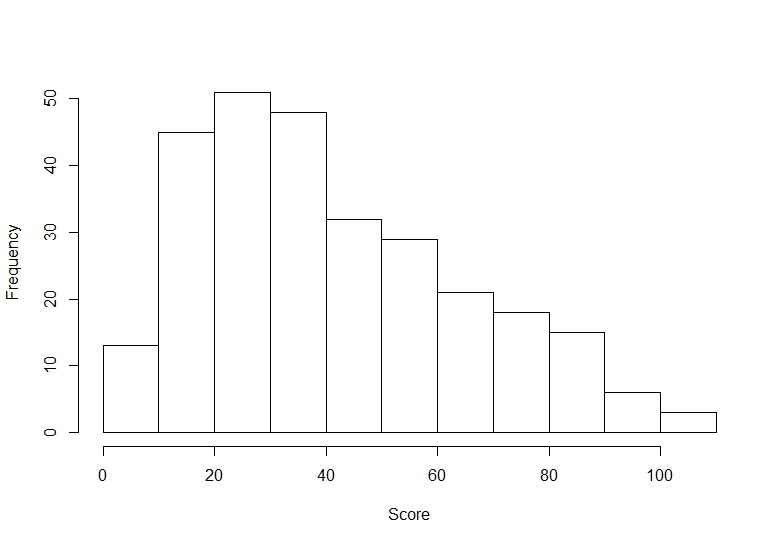
\includegraphics[width=9.5cm]{obr/histogram.png}%
\caption{Score frequency}%
\label{pic:gauss}%
\end{center}
\end{figure}


% Table generated by Excel2LaTeX from sheet 'List1'
\begin{table}[htbp]
  \centering
  \caption{Standardized scores}
	\label{tab:scores}
    \begin{tabular}{lrrrrrrr}
		\hline
    raw&0&20&40&60&80&100&107\\
    \hline
    z&-2.91&-1.00&-0.01&0.67&1.16&2.06&2.91\\
    IQ&56&85&100&110&117&131&144\\
    \hline
    \end{tabular}%
  \label{tab:addlabel}%
\end{table}%


\textbf{Validity}\\
Another question it is important to ask is whether the test is actually measuring the factor it is supposed to measure (i.e. in our case if the score obtained reflects mathematical skills rather than for example the ability to read the question or the writing skill of the examinee). This characteristic is called validity and there are many different ways of proving the test is valid. Most validity proofs come from the outside of the test. One way is to let an examinee to answer a new different test measuring the same factor (ideally a test which is already well established). Another way is to consult other factors known about the examinee, which is what was performed in our case.

As was mentioned above, in addition to solutions to individual problems student's grades from subjects (mathematics, physics, and chemistry) were obtained. It is reasonable to expect a correlation between these grades and the score reached. The correlation is present and its values are shown in the following paragraphs. Because of this fact, although the complete validation would require more thorough examination, it is expected that the test is valid.

\section{Preliminary Test Statistics}
In this section we present an overview of results obtained in testing. This should provide an idea of skills of students, prove validity as mentioned in the paragraph above and will also be referenced later on for comparison.



\begin{table}[htbp]
  \centering
  \caption{Average test scores of the four grammar schools.}
	
	\vspace{3mm}
	
    \begin{tabular}{l|rrrr|r|}
		\hline
    &\textbf{GS1}   & \textbf{GS2} & \textbf{GS3} & \textbf{GS4} & \textbf{Total} \\
					\hline
    &42.76 & 46.68 & 46.35 & 43.65 & 44.53 \\
    \textbf{Males} & 51.40  & 40.08 & 47.77 & 51.03 & 48.48 \\
    \textbf{Females} & 42.53 & 54.86 & 44.45 & 38.81 & 43.06 \\
		\hline
    \end{tabular}%
  \label{tab:totals}%
\end{table}%

The Table~\ref{tab:totals} shows the reached scores divided by gender and school. We calculated Pearson's correlation coefficients of score with other factors. Results are shown in the Table~\ref{tab:corr1}. The correlation test is associated with its p-value, where the null hypothesis is correlation of 0 (no correlation). It means we can say that the correlation between score and all grades (math, physics, and chemistry) is present. The negative value of correlation means that better grade (lower value) yields better score (higher value) which is expected. Furthermore we can see that the grade in mathematics has the highest correlation while physics and chemistry lower. Another significant correlation is interestingly between the fact that the student filled his/her name and his/her score. Positive value shows that those students who filled their name scored better in the test.
On the other hand we can not reject the null hypothesis for gender, so there most likely is no statistically significant correlation between gender and score\footnote{Females were encoded as 1 and males as -1. Negative value would show worst score for females, but it is statistically insignificant.}.

\begin{table}[htbp]%
\caption{Correlations of the score with other factors}
\label{tab:corr1}
\begin{center}
    \begin{tabular}{rrrrrr}
    \hline
    \multicolumn{1}{l}{\textbf{}}  & \multicolumn{1}{l}{\textbf{Gender}} & \multicolumn{1}{l}{\textbf{Mathematics}} & \multicolumn{1}{l}{\textbf{Physics}} & \multicolumn{1}{l}{\textbf{Chemistry}}& \multicolumn{1}{l}{\textbf{Name}} \\
    \hline
    \textbf{Correlation}&  -0.10  & -0.59  & -0.42  & -0.41  & 0.22\\
		\textbf{p-value}&  0.08  & $2.20e^{-16}$  & $3.63e^{-12}$  & $2.65e^{-11}$ & $0.18e^{-4}$ \\
    \hline
    \end{tabular}%
\end{center}
\end{table}

Some questions were in the form of real life problems rather than mathematical problems. These questions were correlated with the score independently as well. The result is displayed in the Table~\ref{tab:corr2}. In the first column it is possible to see that there is a strong and statistically significant correlation of the score obtained in these questions with the total score. Also in this case there is not a strong correlation with the sex of the student even though a bit higher and on the edge of rejection of statistical insignificance. The trend of correlations with grades is preserved but the strength of correlation is lower. In connection with previous results, it leads to an assumption that students with worse grades from these subjects answered correctly rather this kind of questions than other questions.

\begin{table}[htbp]%
\caption{Correlations of the real life problems with other factors}
\label{tab:corr2}
\begin{center}
    \begin{tabular}{rrrrrr}
    \hline
    \multicolumn{1}{l}{\textbf{}} & \multicolumn{1}{l}{\textbf{Score}} & \multicolumn{1}{l}{\textbf{Gender}} & \multicolumn{1}{l}{\textbf{Mathematics}} & \multicolumn{1}{l}{\textbf{Physics}} & \multicolumn{1}{l}{\textbf{Chemistry}} \\
    \hline
    \textbf{Correlation}& 0.69  & -0.19  & -0.38  & -0.25  & -0.27  \\
		\textbf{p-value}& $2.20e^{-16}$   & $0.16e^{-3}$  & $3.16e^{-10}$  & $7.99e^{-5}$   & $2.25e^{-5}$   \\
    \hline
    \end{tabular}%
\end{center}
\end{table}

\chapter{Models for Adaptive Testing}


We remind, as was mentioned in the section~\ref{sec:CATprocess}, the process of an adaptive test.
\begin{enumerate}
	\item The next question to be asked is selected.
	\item The question is asked and a result is obtained.
	\item The result is inserted into the model.
	\item The model (i.e. our estimation about the student) is updated with the result.
	\item (optional) Subsequent answers are estimated / the skill of the student is estimated
\end{enumerate}
In this section we will take a closer look on the model structure for different approaches. Also we will discuss the question selection from step 1 of the list above. Insertion to the model (step 3) and consequent update (steps 4 and 5) of the model is always done with respective standard tools for particular model and will not be extensively discussed here.

\section{Building Models with the Help of IRT}
\label{sec_IRT}
The beginning of Item Response Theory (IRT) appears about 5 decades ago (1968 - Statistical Theories of Mental Test Scores / Lord, Novick -- 1960 - Probabilistic Models for Some Intelligence and..., Rash). This approach is different form the Classical Test Theory (CTT) and it has getting scientific attention ever since [CITACE - str 152].  IRT allows more specific measurement of certain abilities of an examinee. Internationally, there is a large amount of tests adapting this concept. It has stronger assumptions but it also provide stronger results. Nevertheless its spread is not as high as could have been expected. This smaller impact might be caused by the fact that there is a requirement for a stronger statistical and theoretical preparation of a test creator than in the CTT. \textbf{In the Czech Republic there is just a few tests which use this concept. []} 

IRT expects student to have an ability (skill) which directly influences his/her chance of answering a question correctly\footnote{There are variants of multidimensional IRT model where it is possible to have more then one latent variable but in this section we are going to discuss only models with one latent variable.}. This ability is called latent ability or latent trait $\theta$. Every question of the IRT model has associated item response function (IRF) which is a probability of a successful answer given $\theta$. There are more variants to the shape of this IRF but most commonly a 3 parametric model is used (often called 3PL). These parameters reshape a standard logistic function. The resulting IRF, as the probability of a correct answer to \textit{i-th} with the ability of $\theta$, is given by a formula
\begin{equation}
p_i(\theta) = c_i + \frac{1-c_i}{1+e^{-a_i(\theta-b_i)}}
\label{eq:IRF}
\end{equation}
where $c_i$ is a parameter for guessing, $a_i$ sets the scale of the question (this sets its discrimination ability - more steep curve better differentiate between students), $b_i$ is the difficulty of the question (horizontal position of the curve in the space). An example of typical IRFs is shown in the Figure~\ref{pic:IRFs} and the Table~\ref{tab:IRFs} shows their parameters.\\
IRFs are created during the learning procedure of the model from collected data as most likelihood estimates of their parameters.

\begin{figure}
  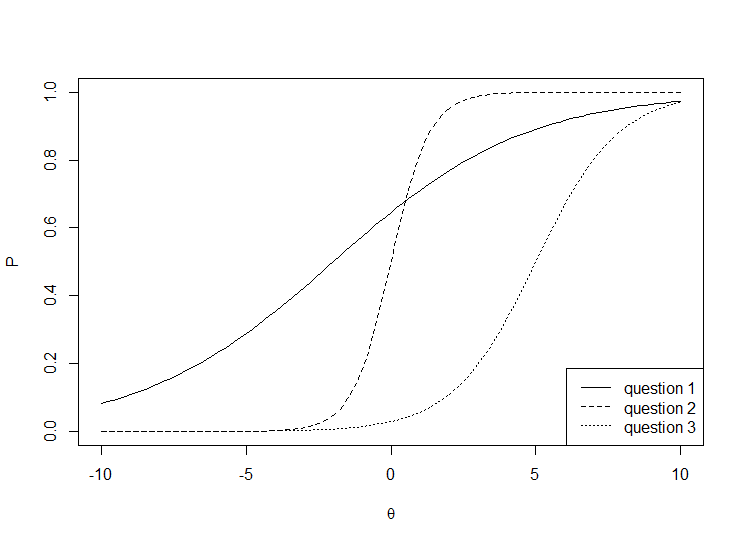
\includegraphics[width=0.8\columnwidth]{obr/irfs.png}%
  \caption{Item Response Functions}%
	\label{pic:IRFs}%
\end{figure}
\begin{table}%
	\begin{tabular}{lccc} \hline
		Question & a & b & c \\ \hline
		1 & -2 & 0.3 & 0\\
		2 & 0 & 1.5 & 0\\
		3 & 5 & 0.7 & 0\\
	\hline
  \end{tabular}
  \caption{IRFs' parameters}%
	\label{tab:IRFs}%
\end{table}
  


\subsection{Adaptive Test Procedure}
Building CAT model with IRT is very straightforward. IRT itself, as was described above, is in the form prepared to be used for CAT. With the model fitted from sample data we have IRFs for every question. In every phase of the test we can compute an estimate of the latent skill $\theta$ based on answers $x$: $p(\theta|x)$. For this estimations Empirical Bayes or Multiple Imputation methods of IRT are used. Knowing the value of the latent skill we know probabilities of correct answers to every question $p_i(\theta)$ and incorrect answers $q_i(\theta)$\footnote{With 3 parametric model these two numbers do not necessarily sum to 1}. More importantly, we are able to calculate the information provided by asking the question. This is called item information and it is given by the formula
$$I_i(\theta)=\frac{(p_i'(\theta))^2}{p_i(\theta)q_i(\theta)}$$
where $p_i'$ is the derivation of the item response function $p_i$. There is an example of typical item information functions (with the same parameters of items as in the Table~\ref{tab:IRFs}) in the Figure~\ref{pic:IG}. This item information provide one, and most straightforward, way of the next question selection. In every step the question $X^*$ which is selected is one with the highest item information. 
$$X^*(\theta) = \arg\max_i I_i(\theta)$$
\textbf{This approach minimizes the standard error of the test procedure.}

\begin{figure}%
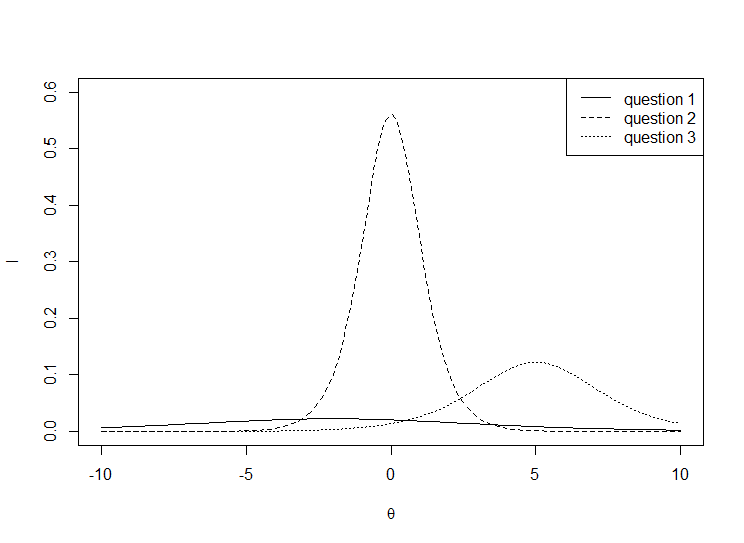
\includegraphics[width=0.8\columnwidth]{obr/IIs.png}%
\caption{Item Information Functions}%
\label{pic:IG}%
\end{figure}

\section{Building Models with the Help of BN}

In this section we go over the basic definitions of Bayesian networks. More theory can be found in []. This section is focused on creation Bayesian networks models for CAT.

Bayesian network is a probabilistic graphical model, a conditional independence structure. It consists of the following: 
\begin{itemize}
	\item a set of variables (nodes),
	\item a set of edges,
	\item a set of conditional probabilities.
\end{itemize}
Edges between variables have to form a directed acyclic graph (DAG). Each variable has a list of mutually exclusive possible states. The conditional probability distribution is defined for each variable conditioned by its parents (variable $A$ with parents $B_1$,$B_2$,...,$B_n$ has the conditional probability table ${P(A|B_1,B_2,...,B_n)}$)\footnote{Note that the variables with no parents have the table in the form $P(A)$}. 

To build a model for adaptive testing as a BN we need to perform 3 steps.
\begin{enumerate}
	\item Describe nodes of the BN
	\item Describe connections between nodes
	\item Initialize conditional probability tables
\end{enumerate}
 
\subsubsection{TYPES OF NODES}
We will divide nodes of a BN into more specific sets. 
\begin{itemize} 
\item A set of $n$ variables we want to estimate $\{S_1,\ldots,S_n\}$. 
We will call them skills or skill variables. We will use symbol $S$ to denote the multivariable $(S_1,\ldots,S_n)$ taking states $s = (s_1,\ldots s_n)$. 
\item A set of $m$ variables representing eventual additional information about the student $\{I_1,\ldots,I_m\}$.  
We will use the symbol $I$ to denote the multivariable $(I_1,\ldots,I_m)$ taking states $i = (i_1,\ldots,i_m)$.
\item A set of $p$ questions (math problems) $\{X_1,\ldots,X_p\}$.  
We will use the symbol $X$ to denote the multivariable $(X_1,\ldots,X_p)$ taking states $x = (x_1,\ldots,x_p)$.
\end{itemize}

\subsubsection{SKILL NODES}
Skill nodes model the student abilities and, generally, they are not directly observable. It means they are hidden variables of the model and their value is not known prior to the model creation. Several decisions are to be made during the model creation.
 
The first decision is the number of skill nodes itself. Should we expect one common skill or should it rather be several different skills each related to a subset of questions only? In the later case it is necessary to specify which skills are required to solve each particular question (i.e. a math problem). 
Skills required for the successful solution of a question become parents of the considered question. This way we create variables with a given meaning (specific student ability). It is not possible to cover all the necessary skills to solve a question. Also there are some other aspect steeping into chances of solving it. During the interpretation of a CAT result we have to be careful. Even though we have given the variable the meaning, it is possible that the model learned a combination of this meaning with other factors. Nevertheless, if the variable was properly constructed it is probable that the most influential one is the correct one.

Another decision we are facing is about the size of a state space of skill nodes. As an unobserved variable, it is hard to decide how many states it should have. Another alternative is to use a continuous skill variable instead of a discrete one but we did not elaborate more 
on this option. For BNs no suitable apparatus to handle continuous parents exists. It would be possible though to create different kind of models with continuous parents other than BNs\footnote{We will elaborate more on this in the last chapter.}. The usage of a discrete state space can be in a way viewed as sampling (or discretizing) the continuous skill variable of the student. It may seem reasonable to do this to many states but each states increases the number of total parameters of the model in a nonlinear way (the exact rate depends on the structure). This means that these models are too complex and it may be very hard to learn them. Conditional probability tables may end up very sparse and that limits the generalization ability of BN. 

States of the skill variable have to be viewed ordinally. It is necessary to order them from the weakest skill to the strongest and this assumption has to hold during the whole process of especially learning and afterwards testing as well. It means, for example, that the probability of 0.5 of a state does tell us the probability of the skill being less or equal than 0.5. If this condition would not be taken into account it may cause inconsistent results. For example a student who is able to answer one very hard question and then fails to answer some easy questions. It would be reasonable to say that the student's ability is somewhere below the middle of its scale. Without the ordinality assumption a BN model could result in probability distribution with peaks at small and high skill levels. It would mean that the student is either good or bad, not mediocre. This does not align with our perception of the student.

\label{observed_score}
It is also possible to replace unobserved skill variables by other observed variables. The easiest way is to introduce score as a variable to the model. To do this it is necessary to use a coarse discretization. At first scores are divided into $n$ equally sized groups and by that we obtain an observed variable having $n$ possible states. The states represent a group of students with similar scores achieved. During the learning phase the variable is observed and the information is used for learning. On the other hand, during the testing, the resulting score is not known -- we are trying to estimate the group into which a test subject falls. In the testing phase the variable is again hidden (unobservable).

Combinations of both types of skill variables are also possible.

\subsubsection{INFORMATION ABOUT A STUDENT}
Information nodes gather any additional information we have about a student. They are observed variables. The number of their states correspond to the possible options of the specific piece of information. One state may be also included as ''unknown'', especially if it holds any information value. For example, for gender we can have 3 states (male, female, unknown). In that case we feel that not knowing itself is an information. Otherwise we would have only two states.
This additional information may improve the quality of the student model. As we discuss in the following chapter, its added value showed up as not very essential. The inclusion of these variables makes the model more complex (more parameters need to be estimated). It may mislead the reasoning by creating prejudices about certain groups of students. The added benefit is low especially in the later stages of testing when sufficient information about a student is collected from his/her answers. 


\subsubsection{QUESTIONS}

The last type of nodes is a question node. This node type holds answers to individual questions. Its state space depends on the number of possible answers to a question. As was mentioned above it is difficult to build a CAT test which does not use multiple choice question type. In some cases it may be possible to have open answers to questions but in most cases these would be too hard to process by the computer system. With multiple choice a question node has two possible state spaces:
\begin{enumerate}
	\item one state for each answer,
	\item one state for correct answer and one for any wrong answer.
\end{enumerate}
The first case is more informative. It gives us a possibility to differentiate between students not only based on the fact that the answer is correct/incorrect but as well on the fact which incorrect one it is. Nevertheless, it has some limitations. The more the states the higher the number of model parameters to be learned. With a limited training data it may be difficult to reliably estimate model parameters. It requires larger data set to learn from. Another aspect is the concept of fairness. It is questionable if it is fair to make distinctions based on wrong answers. On one hand, a classical test usually do not do this. If the answer is wrong then it does not matter which one it is (we can either remove some points from the student's score or not, but it would be the same amount of points for every answer). On the other hand the selected answer shows us some information about the student's ability and there is no theoretical obstacle why not to use it.

\subsubsection{CONNECTIONS BETWEEN NODES}

The next step in the BN model creation is to define a set of arcs between variables (nodes). This set defines relations between skills, questions, and additional information, eventually, also inbetween them.  

\subsection{Model Learning}
The last action to complete a BN is to define conditional probability tables (CPT) for each node. This is done in two steps. In the first one we manually create CPTs (probability of its states given the state of its parent) for every node. Values in these tables should reflect a general expectation and are created with expert knowledge in the field of the test. These probabilities serve as a starting point for the following algorithm. Next we learn the model with standard EM algorithm with collected data. This operation changes values in CPTs to better reflect our specific data.

\subsubsection{TREATING MISSING DATA}
BNs have a large advantage in the way they treat missing data (unknown values). During the prediction process unknown values are simply not inserted into the network and the inference is performed without the knowledge. The learning EM algorithm also has no problems with handling missing data.

\subsection{Adaptive Test Procedure}
During the adaptive test we use standard methods of inference in BNs to update the network. These methods compute estimations of skill variables as well as probabilities of success in unanswered questions.\\
One task to solve during the CAT procedure is the selection of the next question. It is repeated in every step of the testing and it is described below.

Let the test be in the state after $s-1$ steps where 
\begin{eqnarray*}
\mathcal{X}_s & = & \{X_{i_1}\ldots X_{i_n} \ | \ i_1,\ldots,i_n \in \{1,\ldots,m\}\}
\end{eqnarray*}
are unobserved (unanswered) variables and 
\small
\begin{eqnarray*}
\lefteqn{e} &= &\{X_{k_1} = x_{k_1},\ldots,X_{k_o} = x_{k_o} | k_1,\ldots,k_o \in \{1,\ldots,m\}\} 
\end{eqnarray*}
\normalsize
is evidence of observed variables -- questions which were already answered and, possibly, the initial information. 
The goal is to select a variable from $\mathcal{X}_s$ to be asked as the next question. 
We select a question with the largest expected information gain. 

We compute the cumulative Shannon entropy over all skill variables of $S$ given evidence $e$.
It is given by the following formula:
\begin{eqnarray*}
H(e) & = & \sum_{i = 1}^n \sum_{s_i} -P(S_i=s_i|e) \cdot \log P(S_i=s_i|e) \enspace .
\end{eqnarray*}

Assume we decide to ask a question $X' \in \mathcal{X}_s$ with possible outcomes $x'_1,\ldots,x'_p$. 
After inserting the observed outcome the entropy over all skills changes. 
We can compute the value of new entropy for evidence extended by $X' = x_j'$, $j \in \{1,\ldots,p\}$ as:
\begin{eqnarray*}
\lefteqn H(e,X'=x_j') & = & \sum_{i =1}^n \sum_{s_i} \begin{array}{ll}
-P(S_i=s_i|e,X'=x_j')\\
\cdot \log P(S_i=s_i|e,X'=x_j') 
\end{array}\enspace .
\end{eqnarray*}
This entropy $H(e,X'=x_j')$ is the sum of individual entropies over all skill nodes. Another option would be to compute the entropy of the joint probability distribution of all skill nodes. This would take into account correlations between these nodes. In our task we want to estimate marginal probabilities of all skill nodes. In the case of high correlations between two (or more) skills the second criterion would assign them a lower significance in the model. This is the behavior we wanted to avoid. The first criterion assigns the same significance to all skill nodes which seems to us as a better solution. Given the objective of the question selection, the greedy strategy based on the sum of entropies provides good results. Moreover, the computational time required for the proposed method is lower.

Now, we can compute the expected entropy after answering question $X'$: 
\begin{eqnarray*}
EH(X',e) & = & \sum_{j=1}^p P(X'=x_j'|e) \cdot H(e,X'=x_j') \enspace .
\end{eqnarray*}
Finally, we choose a question $X^*$ that maximizes the information gain $IG(X',e)$
\begin{eqnarray*}
X^* & = & \operatorname*{arg\,max}_{X' \in \mathcal{X}_s} IG(X',e) \ , \ \mbox{where}\\
IG(X',e) & = & H(e)  - EH(X',e) \enspace .
\end{eqnarray*}


\subsection{Converting from Skill Node to Score}
\label{sec:converting_skill}
BN models usually produce assumptions about the skills of a student. In some cases this is more useful than a regular score. On the other hand if we want to obtain a score in terms of achieved points we have to transform these skills. It is rather simple for one skill where we introduce a linear transformation from one to another. Basically, we are computing the expected value of the skill variable. The ordering of students stay the same on the score scale as on the expected skill scale. The formula for such a transformation from the skill $S_1$ with states $s_1 \in {1,2,\ldots,n}$ to the score $SC$ is as follows:
$$SC = \sum_{s_1}{P(S_1=s_1|e)\cdot s_1\cdot C} $$
where $C$ is a chosen constant and $e$ is the evidence (answers) of the test. The term $n\cdot C$ is the maximum score because $\sum_{s_1}{P(S_1=s_1|e)} = 1$ and $\underset{s_1}\arg \max (s_1\cdot C) = n$

A problem appears when we need to convert from more than one skill variable. Clearly, we can use the same principle and sum same linear transformations of every skill $S_1,\ldots, S_m$ with states $s_1,\ldots s_m$
\begin{equation}
SC = \sum_{j=1}^m{\sum_{s_j}}{P(S_j=s_j|e)\cdot s_j\cdot C}
\label{eq:scoresum}
\end{equation}

There is a question how large impact should each individual skill variable have on the resulting score. With the formula~\ref{eq:scoresum} the impact depends on the number of states a skill has. It is possible to assign a different scaling factor $C_1,\ldots, C_m$ to each skill variable and the transform the formula~\ref{eq:scoresum} to

\begin{equation}
SC = \sum_{j=1}^m{\sum_{s_j}}{P(S_j=s_j|e)\cdot s_j\cdot C_j} 
\label{eq:scoresum2}
\end{equation}

With $s_{max} = max(s_1,\ldots, s_m)$ and $C_j = \frac{s_{max}}{s_j}\cdot C$ we will assign the same influence to every skill and $C$ is the maximum contribution to the score from each one.

\section{Building Models with the Help of NN}

\subsubsection{TREATING MISSING DATA}
One of the main problems with NNs is the 

\subsection{Selecting Next Question}

\section{Remarks on Models and their Comparison}
Scoring: Both IRT and BN models usually produce assumptions about the skill of a student. There has to be some transformation to the score scale if we want to produce a score of the test. For BN it was discussed in the section~\ref{sec:converting_skill}. NN models does predict the resulting score directly thus there is no conversion needed.\\
Question nodes: BN allow us to exploit every answer to a question as an information about the student. This may help the adaptive test to evolve faster in case there are some answers which are ''more'' wrong that other wrong answers. As was mentioned above it requires large data samples for learning to avoid overfitting.\\
Additional Information: BN and NN models allow us to include additional information about a student. This is not possible in the standard version of IRT-CAT. Inclusion of such additional information may improve prediction power of the model especially during the first stages of the test, but its influence rapidly decrease in the later stages. The use of this information is also questionable in terms of fairness. It may be hard to justify results of the test being influenced by factors other than answers. On the other hand if we want to build a tutoring system, there should be no problem in using it.


\chapter{Experimental Results}
\section{Item Response Theory Model}
\subsection{Model Structure}
\subsection{Testing with IRT}
 
\section{Bayesian Network Model}
\subsection{Model Structure}

\subsection{Testing with BN}

\section{Neural Network Model}
\subsection{Model Structure}
\subsection{Testing with NN}

\section{Models Comparison}
Other than BN models


\chapter*{Conclusions and Future Work} \addcontentsline{toc}{chapter}{Conclusions and Future Work}   
%\input{DP_zaver.tex} 


%%%%%%%%%%%%%%%%%%%%%%  Seznam použitých zdrojů  %%%%%%%%%%%%%%%%%%%%%%
\newpage  % SEM NESAHEJTE!

%LITERATURA

%\newpage % SEM NESAHEJTE!
%%%%%%%%%%%%%%%%%%%%%%  PŘÍLOHY PRÁCE %%%%%%%%%%%%%%%%%%%%%%
%\appendix  % přílohy budou opravdu "Přílohy"  :-)     SEM NESAHEJTE!
%\addcontentsline{toc}{chapter}{Appendix} % přidat položku do obsahu      SEM NESAHEJTE!
%\part*{Appendix}  % SEM NESAHEJTE!
%\input{app1.tex} 

\end{document} % SEM NESAHEJTE!
